% "{'classe':('PSI'),'chapitre':'tec_','type':('application'),'titre':'Tapis de course', 'source':'Pôle Chateaubriand -- Joliot-Curie','comp':('C1-05','C2-08'),'corrige':False}"
%\setchapterimage{bandeau}
\chapter*{Application \arabic{cptApplication} \\ 
Tapis de course -- \ifprof Corrigé \else Sujet \fi}
\addcontentsline{toc}{section}{Application \arabic{cptApplication} : Tapis de course -- \ifprof Corrigé \else Sujet \fi}

\iflivret \stepcounter{cptApplication} \else
\ifprof  \stepcounter{cptApplication} \else \fi
\fi

\setcounter{question}{0}
\marginnote{Pôle Chateaubriand -- Joliot-Curie.}
\marginnote[0cm]{
\UPSTIcompetence[2]{C1-05}
\UPSTIcompetence[2]{C2-08}}

%
%\begin{marginfigure}
%\centering
%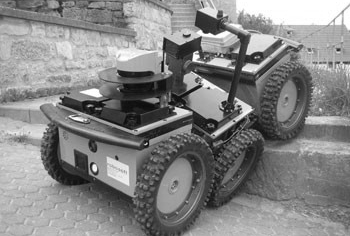
\includegraphics[width=4cm]{fig_00}
%\end{marginfigure}



\ifprof\else
On s’intéresse à un tapis de course dont on
donne une description structurelle ainsi qu’un
extrait de cahier des charges fonctionnel.
L’utilisateur court sur une courroie mobile qui
est entraînée dans le sens inverse de la course.
La vitesse de déplacement de la courroie mobile
est réglable pour permettre au coureur de rester
sur place.
Le système propose un large choix de mode de
fonctionnement cependant l’étude sera limitée
à l’utilisation du programme de contrôle de la
fréquence cardiaque.
Avec ce programme, le système ajuste
automatiquement la vitesse et l’inclinaison du
tapis afin d’obtenir une fréquence cardiaque
préréglée.


\begin{marginfigure}[-1cm]
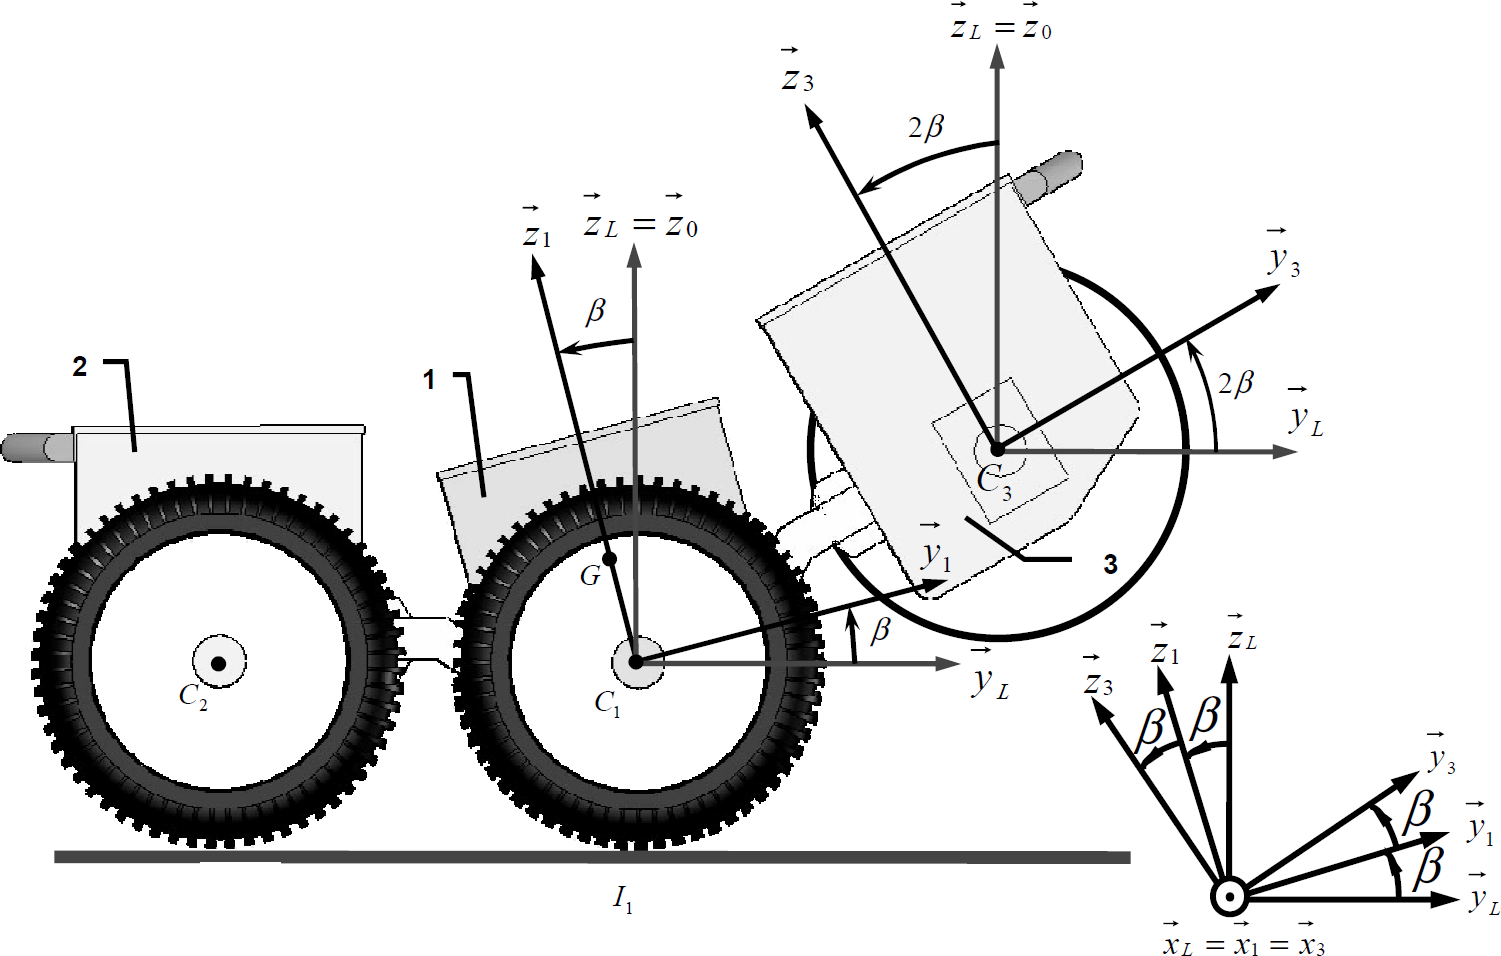
\includegraphics[width=\linewidth]{fig_01_a.png}
\end{marginfigure}




Le programme de contrôle de la fréquence cardiaque fonctionne de la façon suivante :
\begin{itemize}
\item dans un premier temps, le système commence par augmenter la vitesse de déplacement de la courroie
mobile via la chaîne fonctionnelle 1 pour atteindre la fréquence cardiaque préréglée ;
\item si la vitesse maximale ne suffit pas, le tapis de course s’incline via la chaîne fonctionnelle 2 pour
augmenter encore l’effort.
\end{itemize}


%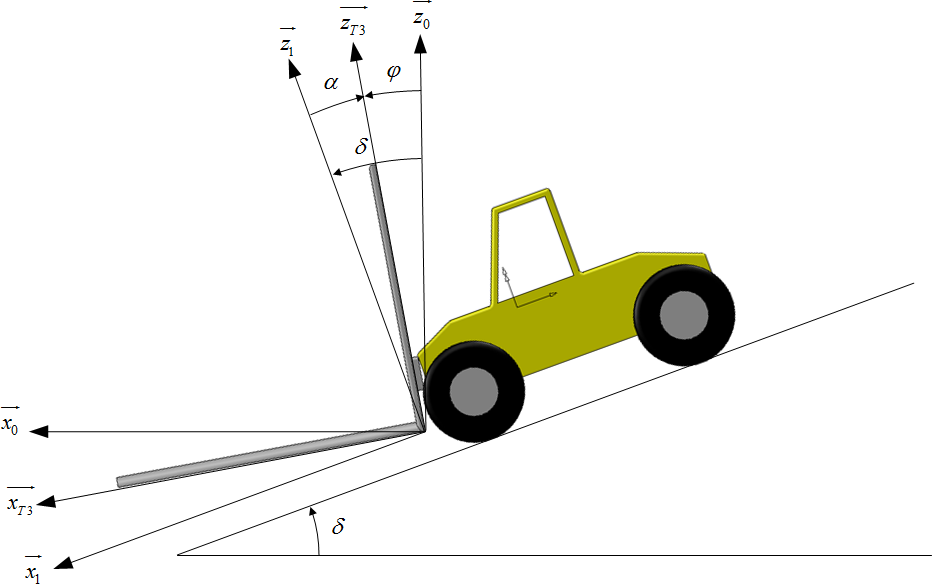
\includegraphics[width=\linewidth]{fig_02.png}

Extrait du cahier des charges :
\begin{table*}[!h]
\centering
\begin{tabular}{p{6cm}p{3cm}p{7cm}}
\hline
\textbf{Exigences} & \textbf{Critères} & \textbf{Niveaux} \\
\hline
\multirow{3}{6cm}{1.1 Le système doit permettre au coureur de courir avec une fréquence cardiaque prédéfiinie.} &
Vitesse de course & De 0 à \SI{19}{km.h^{-1}} par incrément de \SI{0,1}{km.h^{-1}}   \\
& Pente & De 0\, \% à \SI{14}{\%} par incrément de \SI{0,5}{\%}   \\
& Masse utilisateur & \SI{115}{kg} maxi \\
\hline
\end{tabular}
\end{table*}

\begin{marginfigure} 
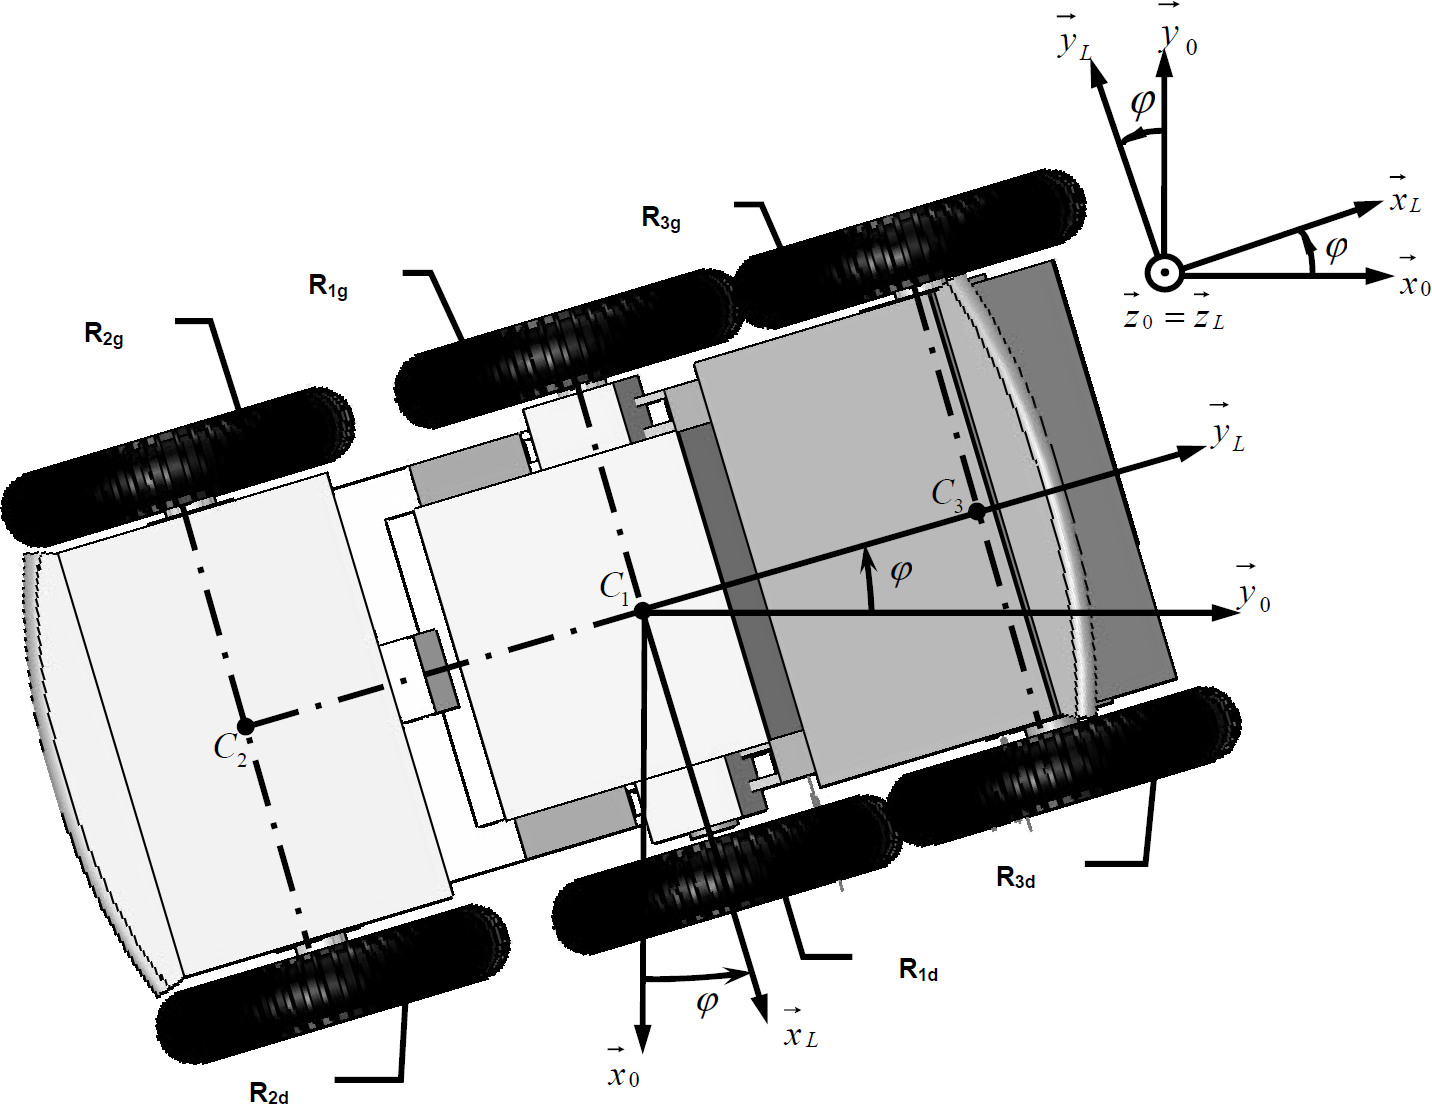
\includegraphics[width=\linewidth]{fig_01_b.png}
\end{marginfigure}
Hypothèses et données :
\begin{itemize}
\item on se place dans le cas où le tapis est réglé à l’horizontale ;
\item la courroie 3, d’épaisseur négligeable, s’enroule sans glisser sur le rouleau 2. Le rayon d’enroulement
de la courroie 3 sur le rouleau 2 est $R_e=\SI{24,5}{mm}$. La poulie 2 est liée au rouleau 2.
\item la courroie 4, d’épaisseur négligeable, s’enroule sans glisser sur les poulies 1 et 2, ainsi que sur le galet.
Les rayons primitifs de la poulie motrice 1 et de la poulie 2 sont respectivement $R_{p1}=\SI{27}{mm}$ et
$R_{p2}=\SI{44}{mm}$;
\item une étude préliminaire a montré que la présence d’un coureur de \SI{115}{kg} entraîne un effort résistant
tangentiel $T_{\text{coureur}\to 3}=\SI{230}{N}$ sur la courroie 3 ;
\item l’inertie équivalente des pièces en mouvement ramenée sur l’arbre moteur est $I_{eq}=\SI{0,1}{kg m^2}$;
\item le rendement global du système mécanique est $\eta=0,9$.
\end{itemize}


\begin{obj}
Valider le choix de la motorisation de la chaîne fonctionnelle 1 vis-à-vis du cahier des charges.
\end{obj}
\fi


\question{Déterminer la vitesse de rotation du moteur $\omega_m$ en rad/s en fonction de la vitesse de déplacement
$V_{30}$ en m/s de la courroie 3. En déduire la vitesse maximale du moteur $\omega_{\text{m max}}$ lorsque la courroie se
déplace à la vitesse maximale indiquée dans le cahier des charges.}
\ifprof
\begin{corrige}
\end{corrige}\else\fi


\question{Déterminer l’expression du couple moteur $C_m$ nécessaire pour mettre en mouvement la courroie 3 en
régime permanent.}
\ifprof
\begin{corrige}
\end{corrige}\else\fi


\question{Déterminer la puissance développée par le moteur lorsque le coureur de \SI{115}{kg} court en régime
établi à \SI{19}{km/h}.}
\ifprof
\begin{corrige}
\end{corrige}\else\fi
Le système possède
un moteur courant
continu ayant les
caractéristiques ci-dessous.

\begin{center}
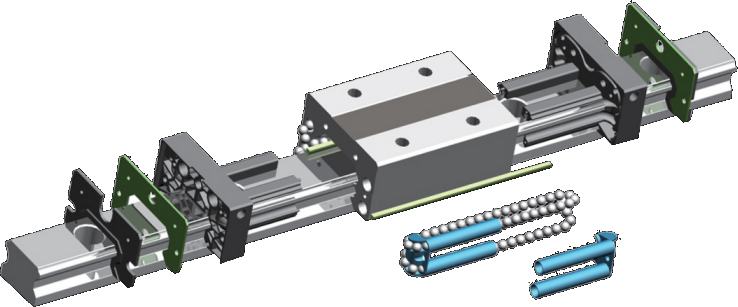
\includegraphics[width=\linewidth]{fig_03.png}
\end{center}

\question{Conclure quant au bon dimensionnement du moteur vis-à-vis des performances attendues.}
\ifprof
\begin{corrige}
\end{corrige}\else\fi

\ifprof
\else
\begin{marginfigure}
\centering

\includegraphics[width=3cm]{Cy_05_01_Application_02_Tapis_qr}
\end{marginfigure}
\fi

\ifcolle
\else
\footnotesize
\marginnote{
\begin{solution}
\begin{enumerate}
\item $\omega_m=\dfrac{R_{p2}}{R_{p1}}\dfrac{V_{30}}{R_e}$ et $\omega_{\text{m max}}=\SI{351}{rad.s^{-1}}$.
\item $C_m=\dfrac{1}{\eta}\left( T_{\text{coureur}\rightarrow 3} R_e \dfrac{R_{p1}}{R_{p2}}\right)$.
\item $P\left(0\to1/0 \right)=\dfrac{1}{0,9}\left(T R_e \dfrac{R_{p1}}{R_{p2}} \right) \omega_{\text{max}}=\SI{1349}{W}$.
\item ...
\end{enumerate}
\end{solution}}
\fi





\ifprof
\begin{center}
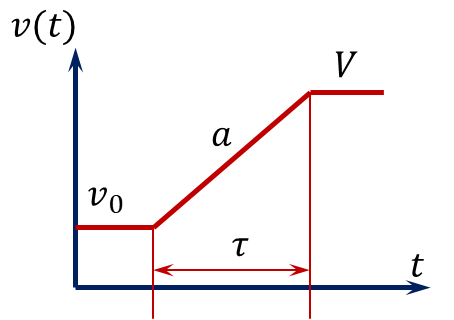
\includegraphics[width=.8\linewidth]{cor_01.png}
\end{center}

\begin{center}
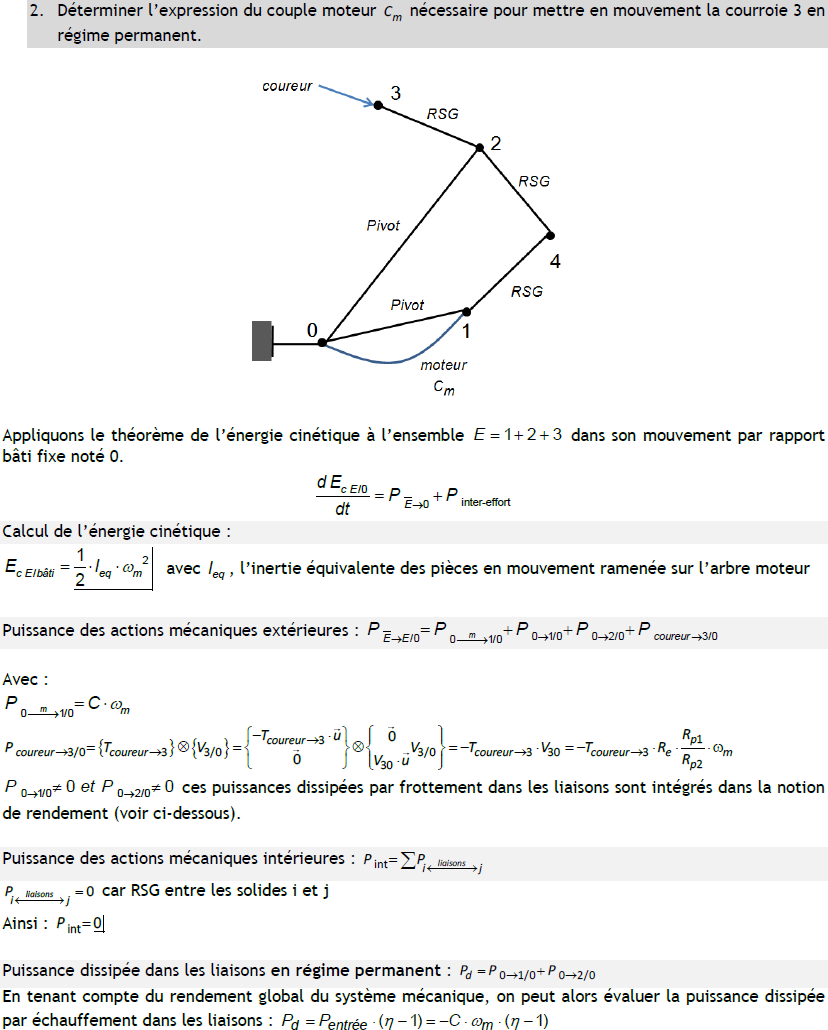
\includegraphics[width=.8\linewidth]{cor_02.png}
\end{center}

\begin{center}
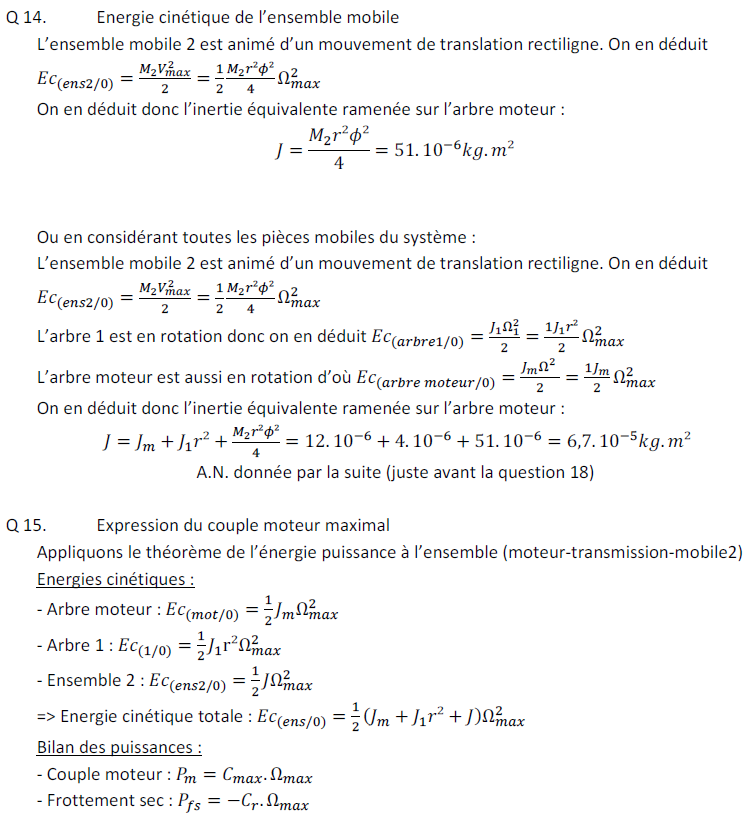
\includegraphics[width=.8\linewidth]{cor_03.png}
\end{center}

\else
\fi